% !TEX TS-program = pdflatex
\documentclass[aspectratio=169]{beamer}
\usepackage[utf8]{inputenc}
\usepackage[T1]{fontenc}
\usetheme{Madrid}
\usecolortheme{seahorse}
\usefonttheme{professionalfonts}
\setbeamertemplate{navigation symbols}{}
\setbeamercovered{transparent}
\setbeamertemplate{itemize items}[circle]
\setbeamertemplate{enumerate items}[default]
\setlength{\parskip}{0.15em}

\definecolor{bepurple}{RGB}{107,63,160}
\definecolor{begold}{RGB}{200,168,75}
\definecolor{beteal}{RGB}{26,122,110}
\definecolor{berust}{RGB}{192,68,42}
\definecolor{beblue}{RGB}{26,74,138}
\definecolor{softpurple}{RGB}{240,232,255}
\definecolor{softgold}{RGB}{255,248,220}
\definecolor{softteal}{RGB}{220,242,240}
\definecolor{softrust}{RGB}{255,235,230}
\setbeamercolor{structure}{fg=beblue}
\setbeamercolor{title}{fg=white,bg=beblue}
\setbeamercolor{frametitle}{fg=beblue}
% Minimal block rendering: regular/example blocks become colored headings (no box)
\setbeamertemplate{block begin}{%
  \par\vspace{0.2ex}%
  \ifx\insertblocktitle\empty\else%
    {\usebeamerfont{block title}\color{beblue}\textbf{\insertblocktitle}}\par\vspace{0.2ex}%
  \fi%
}
\setbeamertemplate{block end}{\par\vspace{0.2ex}}
\setbeamertemplate{block example begin}{%
  \par\vspace{0.2ex}%
  \ifx\insertblocktitle\empty\else%
    {\usebeamerfont{block title}\color{beteal}\textbf{\insertblocktitle}}\par\vspace{0.2ex}%
  \fi%
}
\setbeamertemplate{block example end}{\par\vspace{0.2ex}}
\setbeamertemplate{block alerted begin}{%
  \par\vspace{0.5ex}%
  \begin{beamercolorbox}[sep=0.5ex,rounded=true,shadow=false]{block title alerted}%
    \usebeamerfont{block title}\insertblocktitle%
  \end{beamercolorbox}%
  \nointerlineskip%
  \begin{beamercolorbox}[sep=0.5ex,rounded=true,shadow=false]{block body alerted}%
    \usebeamerfont{block body}%
}
\setbeamertemplate{block alerted end}{\end{beamercolorbox}\par\vspace{0.5ex}}
\setbeamercolor{block title alerted}{fg=white,bg=berust}
\setbeamercolor{block body alerted}{fg=black,bg=berust!8}
\setbeamercolor{alerted text}{fg=berust}

\usepackage{booktabs,amsmath,amssymb,array,multirow,hyperref,colortbl,xcolor}
\usepackage{tikz}
\usepackage{pgfplots}
\pgfplotsset{compat=1.18}
\usetikzlibrary{arrows.meta,positioning,calc,shapes.geometric,patterns}
\hypersetup{colorlinks=true,linkcolor=beblue,urlcolor=beblue}

\title{\textbf{Lecture 8: Behavioural Finance}}
\subtitle{Bubbles, Crashes, Herding, and the Limits of Arbitrage}
\author{Prof.\ Muhebullah Karimzada}
\institute{School of Economics, University of Northern British Columbia}
\date{ECON 230 $\cdot$ Introduction to Behavioural Economics $\cdot$ Winter 2027}

\begin{document}

\begin{frame}[plain]\titlepage\end{frame}

% ============================================================
\begin{frame}{Opening --- The Cisco Impossibility}
\begin{alertblock}{March 2000: Cisco Systems Hits \$555 Billion Market Cap}
To justify this price using standard discounted cash flow analysis:
\begin{itemize}
  \item Cisco needed to grow at \textbf{80\% annually for 10 years}.
  \item Then maintain \textbf{20\% annual growth} indefinitely.
  \item This would make Cisco \textbf{larger than the entire US economy}.
\end{itemize}
\textbf{Did investors know this was impossible? Yes.} \textbf{Did they invest anyway? Yes.}
\end{alertblock}
\begin{block}{The Dot-Com Bubble 2000}
\begin{itemize}
  \item NASDAQ rose \textbf{527\%} from 1995 to March 2000.
  \item NASDAQ then fell \textbf{77\%} from March 2000 to October 2002.
  \item This is what behavioural finance studies: why rational-looking investors create irrational markets.
\end{itemize}
\end{block}
\end{frame}

% ============================================================
\begin{frame}{Lecture Overview}
\begin{enumerate}[<+->]
  \item \textbf{Efficient Market Hypothesis} --- benchmark and evidence for it
  \item \textbf{Anomalies} --- evidence against EMH
  \item \textbf{Limits of Arbitrage} --- why smart money can't always win
  \item \textbf{Noise Traders} --- the model (DeLong et al., 1990)
  \item \textbf{Asset Bubbles} --- anatomy and real examples
  \item \textbf{Herding and Cascades} --- when rational agents create irrational markets
  \item \textbf{Market Anomalies} --- momentum, disposition, home bias
  \item \textbf{2008 Financial Crisis} --- a behavioural post-mortem
  \item \textbf{Canadian housing bubble} (2020--2022) --- close to home
\end{enumerate}
\end{frame}

% ============================================================
\section{The Efficient Market Hypothesis}
% ============================================================

\begin{frame}{The Efficient Market Hypothesis (Fama, 1970)}
All available information is instantly reflected in prices. No strategy can systematically generate \textbf{risk-adjusted abnormal returns}.
\begin{columns}
\column{0.5\textwidth}
\textcolor{beblue}{\textbf{Three Forms:}}
\begin{enumerate}\small
  \item \textbf{Weak:} Past prices don't predict future prices.
  \item \textbf{Semi-strong:} All public info reflected.
  \item \textbf{Strong:} All info (including insider) reflected.
\end{enumerate}
\textcolor{beteal}{\textbf{Evidence FOR:}} 91\% of Canadian active equity funds underperformed over 15 years (SPIVA, 2023). On average, managers \textit{must} earn market return (Sharpe, 1991).
\column{0.47\textwidth}
\begin{alertblock}{But Anomalies Exist}
Momentum, value premium, disposition effect, closed-end fund puzzle, post-earnings drift --- all \textit{systematic} patterns contradicting strict EMH.
\end{alertblock}
\end{columns}
\end{frame}

% ============================================================
\begin{frame}{Noise Trader Model (DeLong et al., 1990)}
Two types: \textbf{rational arbitrageurs} (know fundamentals) and \textbf{noise traders} (trade on sentiment).
\begin{alertblock}{The Surprising Conclusion}
Noise traders can earn \textbf{higher expected returns} because they bear sentiment risk. Rational traders don't fully correct mispricing --- ``markets can stay irrational longer than you can stay solvent.''
\end{alertblock}
\begin{exampleblock}{Limits of Arbitrage (Shleifer \& Vishny, 1997)}
Arbitrage is risky because:
\begin{enumerate}\small
  \item No perfect substitute exists (fundamental risk).
  \item Mispricing can deepen before correcting (noise trader risk).
  \item Arbitrageurs have short horizons and career concerns.
\end{enumerate}
\end{exampleblock}
\end{frame}

% ============================================================
\section{Asset Bubbles}
% ============================================================

\begin{frame}{Historical Bubbles --- A Timeline}
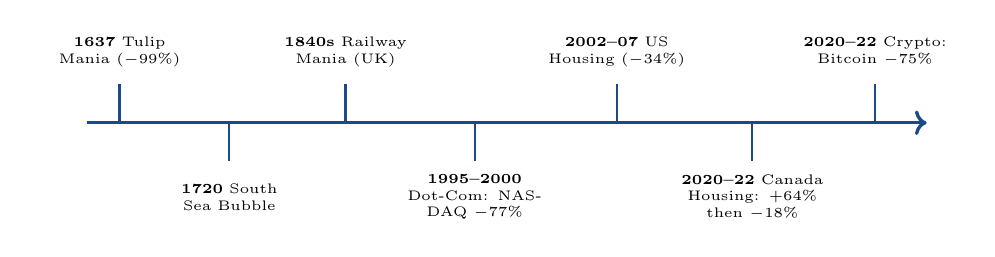
\begin{tikzpicture}[scale=0.82,every node/.style={font=\tiny,align=center,text width=2.1cm}]
  \draw[->,very thick,beblue] (0,0) -- (13,0);
  % Above-timeline items (y > 0)
  \draw[thick,beblue] (0.5,0) -- (0.5,0.6);
  \node at (0.5,1.1) {\textbf{1637} Tulip Mania ($-$99\%)};
  \draw[thick,beblue] (4.0,0) -- (4.0,0.6);
  \node at (4.0,1.1) {\textbf{1840s} Railway Mania (UK)};
  \draw[thick,beblue] (8.2,0) -- (8.2,0.6);
  \node at (8.2,1.1) {\textbf{2002--07} US Housing ($-$34\%)};
  \draw[thick,beblue] (12.2,0) -- (12.2,0.6);
  \node at (12.2,1.1) {\textbf{2020--22} Crypto: Bitcoin $-$75\%};
  % Below-timeline items (y < 0)
  \draw[thick,beblue] (2.2,0) -- (2.2,-0.6);
  \node at (2.2,-1.15) {\textbf{1720} South Sea Bubble};
  \draw[thick,beblue] (6.0,0) -- (6.0,-0.6);
  \node at (6.0,-1.15) {\textbf{1995--2000} Dot-Com: NASDAQ $-$77\%};
  \draw[thick,beblue] (10.3,0) -- (10.3,-0.6);
  \node at (10.3,-1.15) {\textbf{2020--22} Canada Housing: $+$64\% then $-$18\%};
\end{tikzpicture}
\medskip
\begin{block}{Isaac Newton on Tulips (Paraphrased)}
Newton lost £20,000 in the South Sea Bubble (equivalent to $\approx$£3M today): \textit{``I can calculate the motion of heavenly bodies but not the madness of people.''}
\end{block}
\end{frame}

% ============================================================
\begin{frame}{The Dot-Com Bubble}
\begin{columns}
\column{0.52\textwidth}
\begin{tikzpicture}
\begin{axis}[
  width=\textwidth,height=0.55\textheight,
  xlabel={\small Year},ylabel={\small NASDAQ 100 Index},
  xmin=1994,xmax=2005,ymin=0,ymax=5000,
  axis lines=left,
  title={\small NASDAQ 100: 1994--2004}
]
\addplot[beblue,very thick] coordinates{
  (1994,700)(1995,900)(1996,1250)(1997,1800)(1998,2200)(1999,3200)(2000,4700)
  (2001,2200)(2002,1100)(2003,1400)(2004,1900)
};
\node[font=\tiny,berust,fill=softrust,rounded corners] at (axis cs:2000,4900){\textbf{Peak: 4,700}};
\node[font=\tiny,beteal,fill=softteal,rounded corners] at (axis cs:2002,1300){\textbf{Trough: 1,100}};
\draw[<->,berust,thick] (axis cs:2000,4700) -- (axis cs:2002,1100);
\node[font=\tiny,berust] at (axis cs:2001.2,3000){$-$77\%};
\end{axis}
\end{tikzpicture}
\column{0.45\textwidth}
\begin{alertblock}{The Numbers}
\begin{itemize}\small
  \item NASDAQ $+$527\%: 1995 $\to$ 2000; then $-$77\%.
  \item Pets.com: IPO at \$11 $\to$ delisted at \$0.19 (9 months).
  \item Amazon: \$107 $\to$ \$5.97 (2001) before recovering.
\end{itemize}
\end{alertblock}
\textcolor{beblue}{\textbf{Drivers:}} Extrapolation of past returns $\cdot$ ``Tech will change everything'' narrative $\cdot$ Social proof $\cdot$ Overconfidence $\cdot$ Availability bias.
\end{columns}
\end{frame}

% ============================================================
\begin{frame}{The Canadian Housing Bubble (2020--2022)}
\begin{columns}
\column{0.52\textwidth}
\begin{tikzpicture}
\begin{axis}[
  width=\textwidth,height=0.52\textheight,
  xlabel={\small Year},ylabel={\small Price (\$K)},
  xmin=2018,xmax=2024,ymin=400,ymax=900,
  axis lines=left,
  title={\small Canadian Average Home Price}
]
\addplot[beblue,very thick] coordinates{
  (2018,481)(2019,499)(2020,531)(2021,686)(2022.1,820)(2022.5,680)(2023,670)(2024,720)
};
\node[font=\tiny,berust] at (axis cs:2022.2,830){\textbf{\$820K peak}};
\node[font=\tiny,beteal] at (axis cs:2023.2,660){\textbf{$-$18\%}};
\end{axis}
\end{tikzpicture}
\column{0.45\textwidth}
\begin{block}{The Behavioural Story}
\begin{itemize}\small
  \item BoC cut rates to 0.25\% (2020) $\Rightarrow$ prices $+$64\% in 2 years.
  \item \textbf{FOMO}: bought above asking, no conditions.
  \item \textbf{Availability + Extrapolation}: 20 years of rising prices.
\end{itemize}
\end{block}
\begin{alertblock}{The Crash}
\small BoC raised rates to 5.0\% (2022--23). Prices fell \textbf{18\%}. 300K variable-rate holders in payment shock. Loss aversion made sellers resist cuts.
\end{alertblock}
\end{columns}
\end{frame}

% ============================================================
\section{Key Market Anomalies}
% ============================================================

\begin{frame}{The Disposition Effect in Markets}
\begin{block}{Odean (1998) --- US Brokerage Accounts}
Investors are 52\% more likely to sell winning positions than losing positions. The reference point is the purchase price.
\end{block}
\begin{columns}
\column{0.5\textwidth}
\begin{tikzpicture}
\begin{axis}[
  width=\textwidth,height=0.46\textheight,
  ybar,bar width=0.7cm,
  ylabel={\small \% of Positions Sold},
  symbolic x coords={Winners (PGR),Losers (PLR)},
  xtick=data,ymin=0,ymax=20,
  nodes near coords,
  title={\small Disposition Effect (Odean 1998)}
]
\addplot[fill=beteal!70] coordinates{(Winners (PGR),14.8)};
\addplot[fill=berust!70] coordinates{(Losers (PLR),9.8)};
\end{axis}
\end{tikzpicture}
\column{0.47\textwidth}
\begin{alertblock}{Economic Cost}
\begin{itemize}\small\setlength{\itemsep}{0pt}
  \item Stocks sold (winners): earn \textbf{+3.4\%} in next year.
  \item Stocks held (losers): earn \textbf{$-$1.1\%} in next year.
  \item Net annual cost: \textbf{$\approx$4\%} of portfolio value.
  \item Explains momentum anomaly: selling winners $\Rightarrow$ underreaction $\Rightarrow$ continued drift.
\end{itemize}
\end{alertblock}
\end{columns}
\end{frame}

% ============================================================
\begin{frame}{Home Bias}
\begin{columns}
\column{0.5\textwidth}
\begin{tikzpicture}
\begin{axis}[
  width=\textwidth,height=0.7\textheight,
  ybar,bar width=0.35cm,
  ylabel={\small \% of Portfolio in Domestic Stocks},
  symbolic x coords={USA,Canada,Japan,UK,Australia},
  xtick=data,
  x tick label style={font=\tiny},
  ymin=0,ymax=95,
  nodes near coords,
  title={\small Home Bias (French \& Poterba 1991 updated)},
  legend pos=north east
]
\addplot[fill=beblue!70] coordinates{(USA,90)(Canada,50)(Japan,86)(UK,78)(Australia,73)};
\addplot[fill=beteal!70] coordinates{(USA,40)(Canada,3)(Japan,9)(UK,8)(Australia,2)};
\legend{\small Portfolio share,\small World market share}
\end{axis}
\end{tikzpicture}
\column{0.47\textwidth}
\begin{block}{The Puzzle}
Canadian stocks = \textbf{3\%} of world market cap. Canadian investors hold \textbf{50\%} domestic stocks. This is massive over-concentration. Optimal diversification says: hold the world portfolio.
\end{block}
\begin{alertblock}{Behavioural Explanations}
\begin{itemize}\small
  \item \textbf{Familiarity:} invest in what you know (Huberman, 2001).
  \item \textbf{Availability:} Canadian stocks more salient.
  \item \textbf{Overconfidence} + \textbf{Herding} by fund managers.
\end{itemize}
\end{alertblock}
\end{columns}
\end{frame}

% ============================================================
\begin{frame}{Overconfidence and Excess Trading}
\begin{block}{Barber \& Odean (2001) --- ``Boys Will Be Boys''}
Overconfident investors trade more. Overconfidence is higher in men (psychological research). Prediction: men trade more than women and earn less.
\end{block}
\begin{columns}
\column{0.5\textwidth}
\begin{tikzpicture}
\begin{axis}[
  width=\textwidth,height=0.6\textheight,
  ybar,bar width=0.6cm,
  ylabel={\small Annual Turnover / Net Return},
  symbolic x coords={Men Turnover,Women Turnover,Men Return,Women Return},
  xtick=data,x tick label style={font=\tiny,rotate=20,anchor=east},
  ymin=-2,ymax=80,
  nodes near coords,
  title={\small Trading and Returns by Gender}
]
\addplot[fill=beblue!70] coordinates{(Men Turnover,77)(Women Turnover,53)};
\addplot[fill=berust!70] coordinates{(Men Return,-1.4)(Women Return,-0.94)};
\end{axis}
\end{tikzpicture}
\column{0.47\textwidth}
\begin{alertblock}{The Numbers}
\begin{itemize}
  \item Men's annual turnover: \textbf{77\%}
  \item Women's annual turnover: \textbf{53\%}
  \item Men's net annual return: \textbf{$-$1.4\%} vs buy-and-hold
  \item Women's net annual return: \textbf{$-$0.94\%}
  \item Gap: \textbf{0.46\% per year} attributable to overconfidence-driven excess trading
\end{itemize}
\end{alertblock}
\end{columns}
\end{frame}

% ============================================================
\begin{frame}{[GAME] Your Own Portfolio Biases}
\begin{alertblock}{Self-Assessment (Anonymous)}
\begin{enumerate}\small
  \item Ever held a loser to avoid ``locking in a loss''? \textcolor{berust}{$\Rightarrow$ Disposition Effect}
  \item Does your family hold $>$3\% Canadian stocks? \textcolor{berust}{$\Rightarrow$ Home Bias}
  \item Check balances more when markets fall? \textcolor{berust}{$\Rightarrow$ Myopic Loss Aversion}
  \item Changed investment plan after a major market move? \textcolor{berust}{$\Rightarrow$ Availability Bias}
\end{enumerate}
\end{alertblock}
All four are documented in professional money managers and Nobel Prize winners. Not a failure of intelligence --- a predictable consequence of cognitive architecture.
\end{frame}

% ============================================================
\begin{frame}{2008 Financial Crisis --- A Behavioural Post-Mortem}
\begin{block}{Multiple Biases Combined}
\begin{enumerate}[<+->]
  \item \textbf{Overconfidence:} ``Housing prices can only go up'' narrative, widely believed.
  \item \textbf{Availability bias:} 20 years of rising US house prices in memory; no national crash in modern data.
  \item \textbf{Herding:} All major banks held similar MBS exposures simultaneously.
  \item \textbf{Confirmation bias:} Rating agency internal models assumed low default correlations (confirming AAA ratings).
  \item \textbf{Complexity and cognitive overload:} CDO-squared, synthetic CDOs --- opaque to even sophisticated investors.
  \item \textbf{Agency problems:} Mortgage originators bore no default risk.
  \item \textbf{Extrapolation:} Analysts projected historical growth rates into mortgage default models.
\end{enumerate}
\end{block}
\begin{exampleblock}{Canada's Relative Success}
Canada avoided the worst of 2008 due to: strict mortgage underwriting, mandatory CMHC insurance on high-ratio mortgages, no equivalent subprime market. Canadian unemployment peaked at 8.7\% vs US 10\%.
\end{exampleblock}
\end{frame}

% ============================================================
\begin{frame}{Discussion Questions}
\begin{enumerate}
  \item[\textcolor{bepurple}{Q1.}] ``Should retail investors just buy index funds? Is that the behavioural economics prescription?''
  \medskip
  \item[\textcolor{beteal}{Q2.}] ``If you were running a \$1 billion investment fund, what behavioural guardrails would you put in place to prevent your team from falling victim to disposition, herding, and overconfidence?''
  \medskip
  \item[\textcolor{berust}{Q3.}] ``Is it irresponsible for the Bank of Canada to set interest rates knowing that low rates fuel asset bubbles? Should the BoC consider asset prices in its mandate?''
\end{enumerate}
\end{frame}

% ============================================================
\begin{frame}{Key Takeaways --- Lecture 8}
\begin{itemize}
  \item[\textcolor{beteal}{\checkmark}] \textbf{EMH:} compelling benchmark --- 91\% of active Canadian managers underperform. But systematic anomalies exist.
  \item[\textcolor{beteal}{\checkmark}] \textbf{Noise trader model:} rational arbitrageurs can't fully correct mispricing; noise traders can earn higher returns by bearing sentiment risk.
  \item[\textcolor{beteal}{\checkmark}] \textbf{Limits of arbitrage:} fundamental risk, noise trader risk, synchronisation risk, agency costs.
  \item[\textcolor{beteal}{\checkmark}] \textbf{Bubbles:} extrapolation + narrative + herding + overconfidence $\Rightarrow$ prices decouple from fundamentals.
  \item[\textcolor{beteal}{\checkmark}] \textbf{Disposition effect:} sell winners too early, hold losers too long. Costs $\approx$4\%/year.
  \item[\textcolor{beteal}{\checkmark}] \textbf{Home bias:} Canadians hold 50\% domestic despite Canada = 3\% of world market cap.
  \item[\textcolor{beteal}{\checkmark}] \textbf{2008:} overconfidence + herding + extrapolation + complexity $\Rightarrow$ systemic failure.
\end{itemize}
\medskip\textcolor{beblue}{\textbf{Next:}} \textbf{Lecture 9: Nudges \& Choice Architecture} --- We use everything we've learned to improve decisions \textit{without} restricting freedom.
\end{frame}

\end{document}
